\documentclass{article}
\author{Anjal Doshi, Nasser Al-Ghamdi, Nick Rohde}
\title{CSS 534 Program 5 Report}
\date{11$^{th}$ of December 2018}

\usepackage[margin=1in]{geometry} % page margins
\usepackage{graphicx} % images
\graphicspath{ {./images/} } % image path
\usepackage{xcolor} % link colours
\usepackage{hyperref} % links
\usepackage{listings} % code
\usepackage{color} % syntax colours
\usepackage{caption} % figure captions

\definecolor{dkgreen}{rgb}{0,0.6,0}
\definecolor{gray}{rgb}{0.5,0.5,0.5}
\definecolor{mauve}{rgb}{0.58,0,0.82}

\lstset{frame=tb,
	language=Java,
	aboveskip=3mm,
	belowskip=3mm,
	showstringspaces=false,
	columns=flexible,
	basicstyle={\small\ttfamily},
	numbers=none,
	numberstyle=\tiny\color{gray},
	keywordstyle=\color{blue},
	commentstyle=\color{dkgreen},
	stringstyle=\color{mauve},
	breaklines=true,
	breakatwhitespace=true,
	tabsize=2
}

\hypersetup
{
	colorlinks=true,
	citecolor=black,
	filecolor=black,
	linkcolor=black,
	urlcolor=blue,
	linktoc=all,
	linkcolor=blue,
}

\begin{document}
\maketitle
\tableofcontents
\pagebreak
	
	\section{Overview} \label{OVERVIEW}
		Our program five was a parallel implementation of the Simulated Annealing (SA) algorithm. The SA algorithm is a local search based algorithm which uses thermodynamic functions to simulate a system going from a heated state to a cooled state, similar to metal being annealed. The algorithm uses two main loops as part of this simulation. \\
		
		The first of these loops (we will refer to this as the outer loop) simulates the cooling of the system, the initial heat of the system is set to an arbitrary value (in our case 100) and cools until it reaches another arbitrary threshold (in our case 0.001). In this loop we modify the temperature according to equation \hyperref[E_TEMP]{Equation 1} at the conclusion of each iteration. \\
		
		The second loop (we will refer to this as the inner loop) is independent of the heat and is the optimization step, in this loop, we allow the system to stabilize by running a local search for an arbitrary number of iterations (in our case 1,000,000); in this loop, we find a new neighboring solution to our current candidate solution at each step. If a new solution is better than our previous solution, we will always accept it and move our search to its neighborhood; if it is worse, we will calculate an acceptance probability, $p$, using equation \hyperref[E_AP]{Equation 2} and generate a uniformly distributed random number, $r$, if $p > r$ we accept our new (worse) solution, otherwise we reject it. \\
		
		Throughout the process, we keep track of our overall best solution and update it as needed, once the process finishes, this solution is returned as the result.\\
		
		\begin{equation}\label{E_TEMP}
			T(k) = \frac{T(k-1)}{log(k)} \qquad k = annealing~step
		\end{equation}

		\begin{equation}\label{E_AP}
			p(S_i) = e^{-\frac{(-S_{i} + S_{i-1} )}{T}} \qquad S_i = i^{th}~solution; \quad T = current~heat
		\end{equation}
	
	\section{Documentation} \label{DOCUMENTATION}
		\subsection{MPI Java} \label{D_MPI}
			Our MPI Java implementation spread out computation over multiple MPI nodes by running SA on each node individually. \hyperref[F1]{Figure 1} shows a flow diagram of our design. \\
			
			Each node received a different random seed to ensure they did not follow the same path and a different randomly generated starting point. At the conclusion of each outer-loop iteration, all MPI nodes exchange their current best solution and all nodes then adopt the best solution in the cluster. This was done to prevent having nodes follow a dead-end path and keep all nodes searching an area of the search space known to contain good solutions. This can also lead to premature convergence, however, this was the only feasible option we could think of that did not ruin the performance by introducing an immense amount of communication. \\
			
			Furthermore, we divided the number of inner loop iterations over the MPI ranks, i.e. if we ran SA for 100 inner loop iterations over 4 ranks, each rank would only run 25 iterations. This approach is feasible as long as the number of inner loop iterations is sufficiently large. Otherwise it will lead to the algorithm's performance being reduced massively as the system cannot stabilize before the inner loop finishes.\\
		
			\begin{figure}\label{F1}
				\caption{Program Flow of the MPI Implementation.}
				\centering
				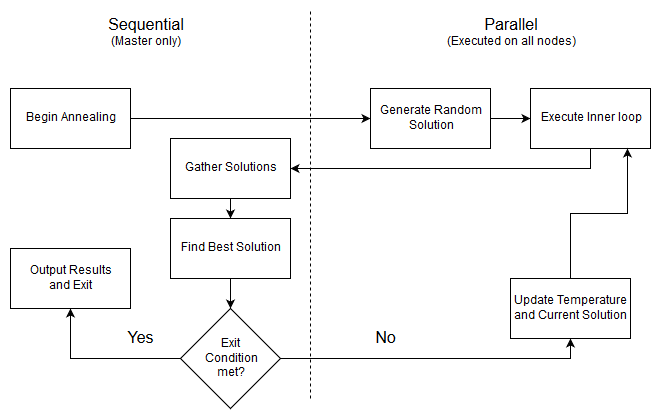
\includegraphics[scale=0.65]{mpi_flow.png}
			\end{figure}
		
		\subsection{MapReduce} \label{D_MR}
		    MapReduce runs the SA algorithm solely in the Mapper. We considered another design where we took the outer loop into the Main function and repeatedly called MapReduce for the inner loop, however, this would have added too much overhead to be feasible. \hyperref[F2]{Figure 2} shows our final design of the MapReduce implementation. \\
			
			We designed the MapReduce algorithm much like the MPI algorithm. Each Mapper receives a line from the input file (each line contains the entire graph) and we control the number of Mapper spawned by MapReduce by adding the graph multiple times to the input file. The Mapper then runs the entire SA algorithm and sends its results to the Reducer. All mappers pass the same key to the Reducer to force all solutions to go to the same Reducer. The Reducer's job is to sift through all solutions and find the best one, which is then returned as the output. \\
			
			\begin{figure}\label{F2}
				\caption{Program Flow of the MapReduce Implementation.}
				\centering
				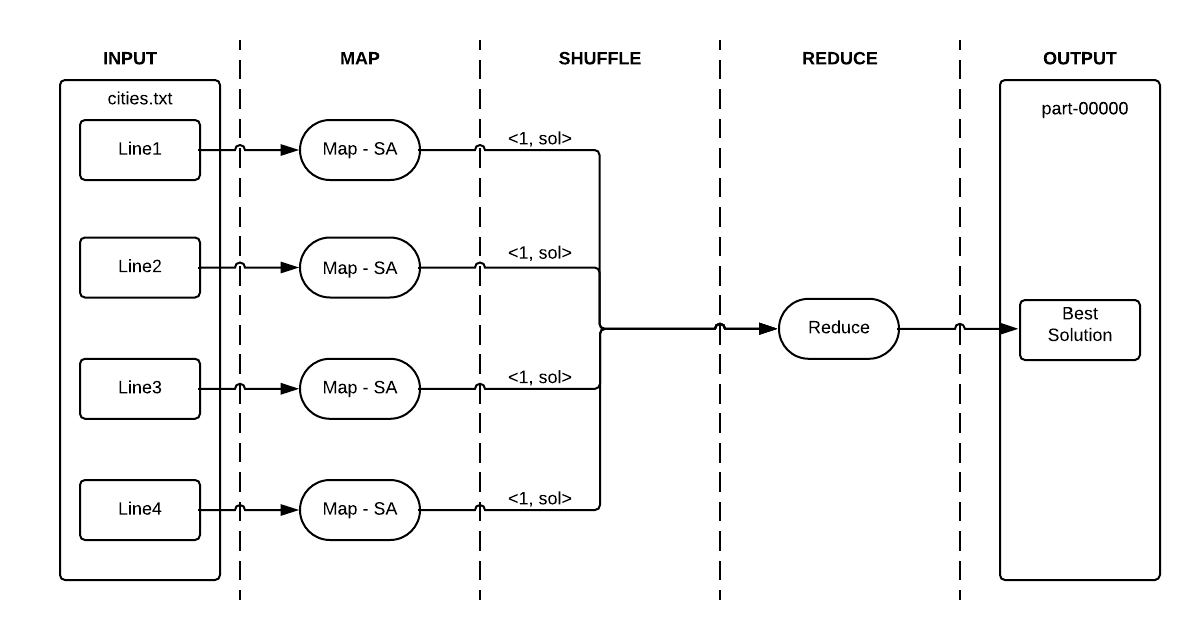
\includegraphics[scale=0.6]{mapreduce_flow.png}
			\end{figure}
		
		\subsection{Spark} \label{D_SPARK}
		The Spark version accepts as additional input the number of partitions. The following steps illustrate the execution process of our Spark implementation:
		\begin{enumerate}
			\item Generate a random initial solution and broadcast it.
			\item Generate a list of 12 (maximum number of executors in the cluster) random number generators, each with a different seed, and broadcast them. Each executor uses its ID to retrieve its generator; thus, each one is extremely unlikely to generate the same solutions as another executor.
			\item Initialize the RDD data structure:
				\begin{itemize} 
					\item Create an initial solution for each partition.
					\item Partition the RDD into the given number of partitions, each containing a single solution.
				\end{itemize}
			\item Run the outer loop (identical to the sequential algorithm):
				\begin{itemize} 
					\item The inner loop uses a map transformation to produce the best solution and the number of iterations is split between the partitions.
				    \item Reduce our solution pool to find the best solution among all partitions.
				    \item Broadcast the best solution.
				\end{itemize}
			\item Output the best solution.
		\end{enumerate}

		\begin{figure}\label{F3}
			\caption{Program Flow of the Spark Implementation.}
			\centering
			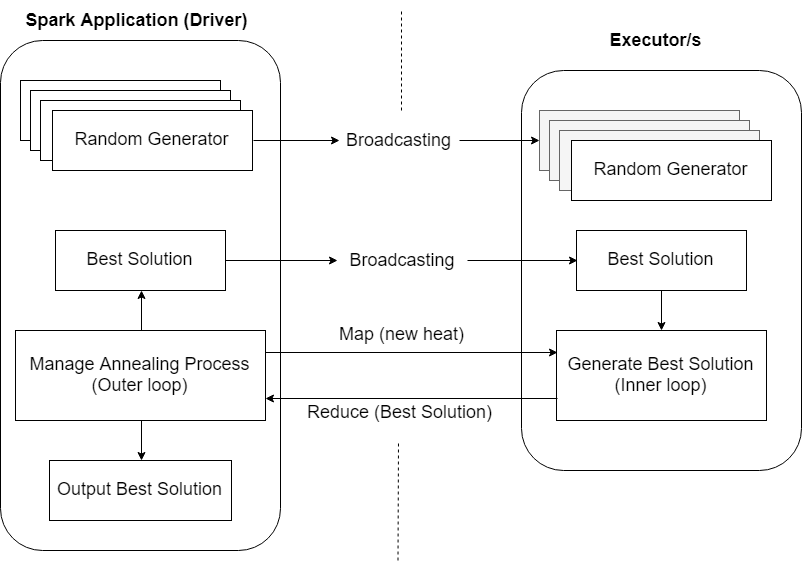
\includegraphics[scale=0.45]{spark_flow_diagram.png}
		\end{figure}
		
		\subsection{MASS} \label{D_MASS}
			Our MASS implementation spread out computation over multiple nodes by creating a Places array where each place was executing the inner loop individually. \\
			
			Each place received a different random seed to ensure they did not follow the same path and a different initial solution. At the conclusion of each outer-loop iteration, all places return their best solution and all these solutions are then filtered for the best overall solution. This solution is then sent to the Places as a starting point for the next iteration of the outer loop. Much like with the MPI version, we split the iterations up between the many MASS nodes, which carries the same drawback as mentioned previously.\\
			
			On unique addition to the algorithm we made in MASS was that we created the number of places equal to the number of running MASS nodes. As MASS assigns each place to a node automatically, we were unable to control how these would be split up over the nodes and hoped that this would encourage MASS to give each node a place. \\

	
	\section{Analysis} \label{ANALYSIS}
        \subsection{Perfromance} \label{PERF}
            In our performance evaluation we considered two scenarios; firstly, we used the input from program 1 with 36 cities scattered throughout the coordinate plane; the other scenario considered 500 equidistant points on a circle with radius 500, thus, all points were almost exactly 2$\pi$ units apart with an optimal trip length of approximately 3641.572 or $1000\pi + 500$, starting at the origin. The optimal trip that we found for the 36 cities was of length $\approx 447.388$, though we have no verification that this is in fact the optimal trip. Our 500 cities example was used as a larger control input with known optimal solution to allow us to analyze how well the different versions of our SA perform with larger input and how close they can get to the best solution.\\
            
            As we can see in \hyperref{T1}{Table 1}, in the 36-city scenario most of our parallel implementations did not manage to beat the sequential program; MPI being the only one with a better performance by a small margin. However, in our larger scenario we see our parallel versions pulling far ahead of the sequential version. The MPI version was able to vastly improve performance here, running almost four times faster than the sequential code. The same applies to MASS, which improved drastically from the 36-city scenario going from 0.326 times to 1.429 times faster execution than sequential. Most likely, MASS could perform better if we used an even larger graph, though we have not tested this; however, MASS's large amount of overhead appears to require a certain amount of minimum execution time to start seeing an improvement in the parallel version. \\
            
            \begin{figure}[!htb] \label{F4}
				\caption{Comparison of Computation for MPI, Spark, MapReduce, and MASS}
				\centering
				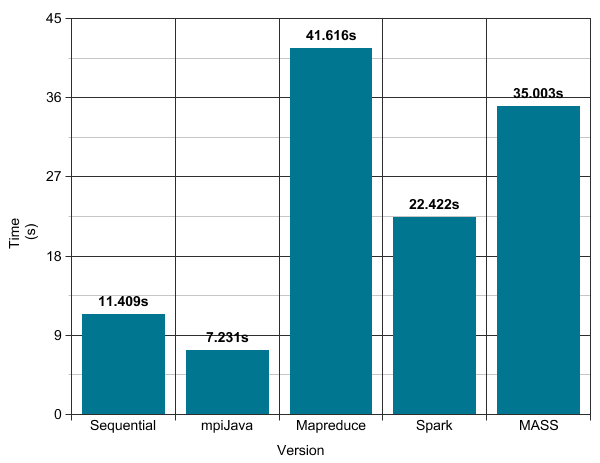
\includegraphics[scale=0.45]{performance_graph.png}
			\end{figure}
			
    		\begin{minipage}{\linewidth}
    			\centering
    			\captionof{table}{Comparison of Computation for MPI, Spark, MapReduce, and MASS} 
    			\begin{tabular}{c|cc|cc}\label{T1}
    				& \multicolumn{2}{c|}{36 Cities} & \multicolumn{2}{c}{500 Cities} \\
    				Version & Execution Time (s)$^{\dagger}$ & Improvement 	& Execution Time (s) 	& Improvement\\
    				\hline
    				Sequential	& 11.409	& N/A			& 157.222	& N/A	\\
    				MPI Java 	&  7.231	& 1.578			&  39.627	& 3.968	\\
    				MapReduce	& 41.616	& 0.274			& TODO		& TODO \\
    				Spark		& 22.422	& 0.509			& TODO		& TODO \\
    				MASS		& 35.003	& 0.326			& 109.998	& 1.429 \\
    				\noalign{\smallskip}\hline\noalign{\smallskip}
    				\multicolumn{3}{l}{\tiny $^\dagger$ Time of the best performing configuration of the given SA version.}
    			\end{tabular}
    			\smallskip\smallskip\smallskip\smallskip
    		\end{minipage}
        
            \subsubsection{MPI JAVA} \label{PER_MPI}
				Looking at \hyperref{T2}{Table 2}, we can see that our MPI program is performing very well in terms of performance scaling, in fact, we experience over 4.5 times execution time improvement when comparing a single vs four MPI nodes. When we look at \hyperref{T1}{Table 1}, we can see that MPI with four nodes is able to keep up with the sequential version of the algorithm, but not able to beat it by a large margin. One explanation for this is that the problem is not complex enough for the communication overhead to become negible. However, comparing MPI to the other three solutions, we can see a very different result. We believe that our tight control over communication in MPI is responsible for our MPI version performing so much better than the MapReduce, Spark, and MASS versions. As MPI conducts no communication unless specifically told by the programmer, we can ensure that we only communicate when absolutely necessary, allowing us to optimize the performance the most. \\
	
            
        		\begin{minipage}{\linewidth}
        			\centering
        			\captionof{table}{Comparison of Computation for MPI} 
        			\begin{tabular}{c|cc|cc}\label{T2}
        				& \multicolumn{2}{c|}{36 Cities} & \multicolumn{2}{c}{500 Cities} \\
        				\# Nodes & Average Execution Time (s)$^{\dagger}$ 	& Improvement & Execution Time (s) & Improvement \\
        				\hline
        				1		& 32.8419	& N/A		& 155.536	& N/A 	\\
        				2		& 16.0231	& 2.050		&  77.738	& 2.000	\\
        				4		&  7.2312	& 4.542		&  39.627	& 3.925 \\
        			\noalign{\smallskip}\hline\noalign{\smallskip}
        			\multicolumn{3}{l}{\tiny $^\dagger$ Average over 100 trials}
        			\end{tabular}
        		\smallskip\smallskip\smallskip\smallskip
        		\end{minipage}
            
            \subsubsection{MapReduce} \label{PER_MR}
        		\begin{minipage}{\linewidth}
                    \centering
        			\captionof{table}{Comparison of Computation for MapReduce} 
        			\begin{tabular}{c|cc|cc}\label{T3}
        				& \multicolumn{2}{c|}{36 Cities} & \multicolumn{2}{c}{500 Cities} \\
        				\# Nodes & Execution Time (s) & Improvement & Execution Time (s) & Improvement \\
        				\hline
        				1	& 55.972	& N/A	&	TODO	& N/A \\
        				2	& 41.616	& 1.345	&	TODO	& TODO \\
        				4	& 44.423	& 1.256 &	TODO	& TODO \\
        			\end{tabular}
        		\smallskip\smallskip\smallskip\smallskip
                \end{minipage}
                
                MapReduce is designed to work efficiently with Big Data. In our algorithm the input data is tiny. The main focus is the iterative computation of intermediate solution. Such algorithms are not not the best choice to be implemented in MapReduce. Which results in the performance to be significantly lower than the sequential version. One way the performance could be improved is by making the number of cities in the input file very large. This would definitely show better performance than the sequential version.\\
            
            \subsubsection{Spark} \label{PER_SPARK}
        		\begin{minipage}{\linewidth}
        			\centering
        			\captionof{table}{Comparison of Computation for Spark} 
        			\begin{tabular}{c|cc|cc}\label{T4}
        				& \multicolumn{2}{c|}{36 Cities} & \multicolumn{2}{c}{500 Cities} \\
        				\# Nodes  & Execution Time (s) 	& Improvement & Execution Time (s) 	& Improvement	\\
        				\hline
        				1	& 36.866	& N/A	&	362.796	& N/A \\
        				2	& 23.620	& 1.56	&	90.352	& 4.015 \\
        				4	& 22.422 	& 1.644	&	85.542	& 4.241 \\
        			\end{tabular}
        		\smallskip\smallskip\smallskip\smallskip
				\end{minipage}

				In Spark, the user cannot assign a specific task to a designated node; in other words, the number of tasks and the executor of a given task is managed by the DAG-Scheduler and Task Scheduler. For this reason, we used partitions to ensure there will be at least the same number of tasks as nodes in the cluster to utilize all computational resources available. The number of partitions changes based on the number of nodes in the cluster.\\
    		
    		\subsubsection{MASS} \label{PER_MASS}
        		\begin{minipage}{\linewidth}
                    \centering
        			\captionof{table}{Comparison of Computation for MASS} 
        			\begin{tabular}{c|cc|cc}\label{T5}
        				& \multicolumn{2}{c|}{36 Cities} & \multicolumn{2}{c}{500 Cities} \\
        				\# Nodes & Execution Time (s) & Improvement & Execution Time (s) & Improvement\\
        				\hline
        				1	& 35.003	& N/A	&	321.528	& N/A \\
        				2	& 41.684	& 0.839 &	189.145	& 1.700 \\
        				4	& 58.490	& 0.598 &	109.998	& 2.923 \\
        			\end{tabular}
        		\smallskip\smallskip\smallskip\smallskip
                \end{minipage}
            
            	Our performance with MASS in the 36-city scenario created some rather strange results, as our execution time actually increased with more programming nodes. We hypothesized that this was due to the communication overhead. After running MASS on the 500-city scenario, this hypothesis seems to be supported, as our execution time now did what was expected and decreased as we added nodes. However, it appears that MASS still has too much overhead to be feasible for such a simple problem as all our other approaches still beat it by a wide margin in the 500-city scenario. \\
		
		\subsection{Programmability} \label{PROG}
			The programmability differed vastly between the different strategies that we used. \\
			
			MPI makes it very easy to turn a sequential program into a parallel one and presented little problems for us. Furthermore, MPI allows us to have tight control over communication, allowing us to optimize our program more than the other versions did.\\
			
			Similarly, Spark also made it quite simple to program our SA algorithm and we had little issues to convert the sequential code into a parallel version. Spark presented some challenges in ensuring our random number generators were seeded correctly to prevent all executors from doing the same thing, however, it was not difficult to find a way to implement this using the ExecutorID in the SparkConf object. \\
			
			MapReduce, on the other hand, presented a bigger challenge due to the Hadoop file-system. First of all, we had to come up with a work around of starting our Mappers appropriately to ensure they all received the entire graph. As our graph was on multiple lines, we had to put our entire graph on a single line to ensure each Mapper receives the whole graph and not just a single city. Furthermore, MapReduce makes it challenging to communicate between Mapper and Reducer, therefore we had to do all work in the Mapper with the Reducer doing basically nothing. It has to be said that this was partly because of our problem, SA was simply not a good algorithm for MapReduce.\\
			
			Lastly, MASS presented a number of challenges for us as well. One of the main problems we had with it was the fact that it is very particular about the configurations in the nodes.xml document. Generally, we expect that if we tell java to run a given class, it will use the path that we gave it, however, MASS actually looks in the MASS home for files in the worker nodes, instead of passing the correct path to the workers. This made it somewhat challenging to run our code. However, the biggest challenge with MASS was the awful documentation that accompanies it. The documentation does not adequately explain what can and cannot be done with MASS or exactly how to use MASS. A good example would be passing multiple arguments to the callAll function. We assumed that we could pass an Object array to this method and this would be passed on to our function. However, this was not the case, so we were required to build a wrapper class to hold our arguments for the callAll call, which we then needed to unpack in the callAll function. This added unnecessary boilerplate code and complexity to our program. \\
			 
			Overall, the programmability of these four libraries was acceptable and most of them did not require too much boilerplate code to be added to use the library. MapReduce and Mass required the most boilerplate code to make the program work, with Spark requiring virtually nothing. MPI ended up in the middle of the pack as our program involved only a small amount of communication. \\
		
        		\begin{minipage}{\linewidth}
                    \centering
        			\captionof{table}{Comparison of Boilerplate Calls} 
        			\begin{tabular}{c|cccc}\label{T6}
        				Version 	& \# of Classes & Lines of Boilerplate Code & Total \# Lines & Boilerplate \%\\
        				\hline
        				Sequential	& 4		& N/A	& 104 	& N/A 	\\
        				MPI			& 6		& 18	& 137 	& 13.14 \\
        				MapReduce	& 6		& 19	& 141	& 13.48	\\
        				Spark		& 5		& 4		& 128	&  3.13	\\
        				MASS		& 6		& 47	& 135	& 34.81	\\
        				\hline
        				Mean: 		& 5.4	& 22	& 129	& 16.14	\\
        			\end{tabular}
        		\smallskip\smallskip\smallskip\smallskip
                \end{minipage}


\pagebreak
	
	\section{Source Code} \label{SRC}
		\subsection{Program 5} \label{P5_SRC}
		The source codes for Program 5 can be found in the included src folder.\\
	
	
		\subsection{Laboratory 5} \label{L5_SRC}
			The source code for laboratory 5 is shown below and is also in the included src folder.\\
			For our laboratory, we modified the Matrix, Nomad, and QuickStart classes to build a 2D Places of size 10 x 10, populated with 10 Agents that moved through the Places migrate according to the function: $x_{new} = x_{old} * 8 + 2$ and $y_{new} = y_{old} * 2 - 4$.
			\begin{lstlisting}
			\* Agent Class *\
public class AgentX extends Agent {

	public static final int GET_HOSTNAME = 0;
	public static final int MIGRATE = 1;
	
	
	/**
	* This constructor will be called upon instantiation by MASS
	* The Object supplied MAY be the same object supplied when Places was created
	* @param obj
	*/
	public AgentX(Object obj) { }
	
	/**
	* This method is called when "callAll" is invoked from the master node
	*/
	public Object callMethod(int method, Object o) {
		switch (method) {
			case GET_HOSTNAME:
				return findHostName(o);
			case MIGRATE:
				return move(o);		
			default:
				return new String("Unknown Method Number: " + method);
		}
	}
	
	/**
	* Return a String identifying where this Agent is actually located
	* @param o
	* @return The hostname (as a String) where this Agent is located
	*/
	public Object findHostName(Object o){
		try{
			return (String) "Agent located at: " + InetAddress.getLocalHost().getCanonicalHostName() + " " + Integer.toString(getIndex()[0]) + ":" + Integer.toString(getIndex()[1]) + ":" + Integer.toString(getIndex()[2]);
		}catch(Exception e) {
			return "Error : " + e.getLocalizedMessage() + e.getStackTrace();
		}    
	}
	
	/**
	* Move this Agent to the next position in the X-coordinate
	* @param o
	* @return
	*/
	public Object move(Object o) {
	
		int xModifier = this.getPlace().getIndex()[0] * 8 + 2;
		int yModifier = this.getPlace().getIndex()[1] * 2 - 4;	        
		
		migrate(xModifier, yModifier);
		return o;
	}
}
			
			
			\* Places Class *\
			
public class Coords extends Place {
	public static final int GET_HOSTNAME = 0;
	
	/**
	* This constructor will be called upon instantiation by MASS
	* The Object supplied MAY be the same object supplied when Places was created
	* @param obj
	*/
	public Coords(Object obj) { }
	
	/**
	* This method is called when "callAll" is invoked from the master node
	*/
	public Object callMethod(int method, Object o) {
		switch (method) {
		case GET_HOSTNAME:
			return findHostName(o);
		default:
			return new String("Unknown Method Number: " + method);
		}
	}
	
	/**
	* Return a String identifying where this Place is actually located
	* @param o
	* @return The hostname (as a String) where this Place is located
	*/
	public Object findHostName(Object o){
	
		try{
			return (String) "Place located at: " + InetAddress.getLocalHost().getCanonicalHostName() +" " + Integer.toString(getIndex()[0]) + ":" + Integer.toString(getIndex()[1]) + ":" + Integer.toString(getIndex()[2]);
		}catch (Exception e) {
			return "Error : " + e.getLocalizedMessage() + e.getStackTrace();
		}
	}
}		


			\* Main Class *\
			
public class Main {
	private static final String NODE_FILE = "nodes.xml";	
 
	public static void main( String[] args ) {
		// remember starting time
		long startTime = new Date().getTime();
		
		// init MASS library
		MASS.setNodeFilePath( NODE_FILE );
		MASS.setLoggingLevel( LogLevel.DEBUG );
		
		// start MASS
		MASS.init();
		
		int x = 10;
		int y = 10;

		// initialize a 2D places object
		Places places = new Places( 1, Coords.class.getName(), ( Object ) new Integer( 0 ), x, y );
		
		// initialize some Agents
		Agents agents = new Agents( 1, AgentX.class.getName(), null, places, x);

		// instruct agents to move once
		agents.callAll(AgentX.MIGRATE);
		agents.manageAll();

		// stop MASS
		MASS.finish();
		
		// calculate / display execution time
		long execTime = new Date().getTime() - startTime;
		System.out.println( "Execution time = " + execTime + " milliseconds" );
	}
}
			
			
			\end{lstlisting}
			
	
	\section{Output} \label{OUT}
	
		\subsection{Program 5} \label{P5_OUT}		
			\begin{lstlisting}
/** Sequential Program **/
java SA 1000000 ../input_files/cities.txt
Best solution found:path: 21 -> 27 -> 24 -> 25 -> 7 -> 31 -> 2 -> 22 -> 18 -> 12 -> 15 -> 28 -> 26 -> 4 -> 20 -> 9 -> 32 -> 14 -> 8 -> 34 -> 30 -> 19 -> 13 -> 23 -> 6 -> 10 -> 35 -> 5 -> 0 -> 11 -> 33 -> 17 -> 29 -> 3 -> 1 -> 16 | distance: 447.38786463942176
Elapsed time:11409 ms.

java SA 1000000 ../input_files/graph3.txt
Best solution found:path: 483 -> 484 -> 485 -> 486 -> 487 -> ... 445 -> 444 -> 443 -> 442 -> 441 | distance: 12633.601936741623
Elapsed time:157222 ms.

--------------------------------------------

/** MPI Program **/
run_mpi 4 Runner 2000000 ../input_files/cities.txt
Solution is:path: 21 -> 27 -> 24 -> 25 -> 7 -> 31 -> 2 -> 22 -> 18 -> 12 -> 15 -> 28 -> 26 -> 4 -> 20 -> 9 -> 32 -> 14 -> 8 -> 34 -> 30 -> 19 -> 13 -> 23 -> 6 -> 10 -> 35 -> 5 -> 0 -> 11 -> 33 -> 17 -> 29 -> 3 -> 1 -> 16 | distance: 447.38786463942176
Execution time: 7898 ms.

run_mpi 4 Runner 1000000 ../input_files/graph3.txt
Solution is:path: 370 -> 369 -> 368 -> 367 -> 366 -> ... 284 -> 285 -> 286 -> 287 -> 288 | distance: 14940.310162436743
Execution time: 39627 ms.

-------------------------------------------

/** MapReduce Program **/
hadoop jar TspRunner.jar TspRunner 1000000 input output
Execution Time: 42553ms

hadoop fs -cat /user/anjald_css534/output/part-00000
Best Solution Found:    path: 21 -> 27 -> 24 -> 25 -> 7 -> 31 -> 2 -> 22 -> 18 -> 12 -> 15 -> 28 -> 26 -> 4 -> 20 -> 9 -> 32 -> 14 -> 8 -> 34 -> 30 -> 19 -> 13 -> 23 -> 6 -> 10 -> 35 -> 5 -> 0 -> 11 -> 33 -> 17 -> 29 -> 3 -> 1 -> 16 | distance: 447.38786463942176

--------------------------------------------

/** Spark Program **/
spark-submit --class uwb.css534.prog5.App --master "spark://cssmpi1.uwb.edu:60007" --total-executor-cores 12 sa-tsp-spark-1.0-SNAPSHOT.jar 2000000 CSS534_Program5/code/input_files/cities.txt 12
Best solution found:path: 21 -> 27 -> 24 -> 25 -> 7 -> 31 -> 2 -> 22 -> 18 -> 12 -> 15 -> 28 -> 26 -> 4 -> 20 -> 9 -> 32 -> 14 -> 8 -> 34 -> 30 -> 19 -> 13 -> 23 -> 6 -> 10 -> 35 -> 5 -> 0 -> 11 -> 33 -> 17 -> 29 -> 3 -> 1 -> 16 | distance: 447.38786463942176
Elapsed time:22422 ms.

spark-submit --class uwb.css534.prog5.App --master "spark://cssmpi1.uwb.edu:60007" --total-executor-cores 12 sa-tsp-spark-1.0-SNAPSHOT.jar 10000000 CSS534_Program5/code/input_files/cities.txt 100
Best solution found:path: 21 -> 27 -> 24 -> 25 -> 7 -> 31 -> 2 -> 22 -> 18 -> 12 -> 15 -> 28 -> 26 -> 4 -> 20 -> 9 -> 32 -> 14 -> 8 -> 34 -> 30 -> 19 -> 13 -> 23 -> 6 -> 10 -> 35 -> 5 -> 0 -> 11 -> 33 -> 17 -> 29 -> 3 -> 1 -> 16 | distance: 447.38786463942176
Elapsed time:29135 ms.
--------------------------------------------

/** MASS Program **/
java -jar prog5-1.0-SNAPSHOT.jar 2000000 cities.txt 4
MProcess on v0243p.host.s.uw.edu run with command: java -Xmx9g -cp /home/anjald_css534/prog5/.jar edu.uw.bothell.css.dsl.MASS.MProcess v0243p.host.s.uw.edu 1 4 1 58136 /home/anjald_css534/prog5
MProcess on v0244p.host.s.uw.edu run with command: java -Xmx9g -cp /home/anjald_css534/prog5/.jar edu.uw.bothell.css.dsl.MASS.MProcess v0244p.host.s.uw.edu 2 4 1 58136 /home/anjald_css534/prog5
MProcess on v0245p.host.s.uw.edu run with command: java -Xmx9g -cp /home/anjald_css534/prog5/.jar edu.uw.bothell.css.dsl.MASS.MProcess v0245p.host.s.uw.edu 3 4 1 58136 /home/anjald_css534/prog5
MASS.init: done
Best Solution:path: 21 -> 27 -> 24 -> 25 -> 7 -> 20 -> 4 -> 26 -> 28 -> 31 -> 2 -> 22 -> 18 -> 12 -> 15 -> 16 -> 1 -> 3 -> 29 -> 17 -> 33 -> 11 -> 0 -> 5 -> 35 -> 10 -> 6 -> 23 -> 13 -> 19 -> 30 -> 34 -> 8 -> 14 -> 32 -> 9 | distance: 449.6584675618958
Execution time = 57156 milliseconds


			\end{lstlisting}	
	
\end{document}